% This is samplepaper.tex, a sample chapter demonstrating the
% LLNCS macro package for Springer Computer Science proceedings;
% Version 2.20 of 2017/10/04
%
\documentclass[runningheads]{llncs}
%
\usepackage{graphicx}
\usepackage{tabularx}
\usepackage{hyperref}
% Used for displaying a sample figure. If possible, figure files should
% be included in EPS format.
%
% If you use the hyperref package, please uncomment the following line
% to display URLs in blue roman font according to Springer's eBook style:
% \renewcommand\UrlFont{\color{blue}\rmfamily}

\begin{document}
%
\title{Navigating the Bumpy Road from Engineer to Manager}
%
%\titlerunning{Abbreviated paper title}
% If the paper title is too long for the running head, you can set
% an abbreviated paper title here
%
\author{Shubham Vipulkumar Patel\inst{1}
% \and
% Second Author\inst{2,3}\orcidID{1111-2222-3333-4444} \and
% Third Author\inst{3}\orcidID{2222--3333-4444-5555}
}
%
\authorrunning{F. Author et al.}
% First names are abbreviated in the running head.
% If there are more than two authors, 'et al.' is used.
%
% \institute{Concordia University, Montreal QC, Canada \and
% Springer Heidelberg, Tiergartenstr. 17, 69121 Heidelberg, Germany
% \email{lncs@springer.com}\\
% \url{http://www.springer.com/gp/computer-science/lncs} \and
% ABC Institute, Rupert-Karls-University Heidelberg, Heidelberg, Germany\\
% \email{\{abc,lncs\}@uni-heidelberg.de}}
\institute{Concordia University, Montreal QC, Canada\\
\email{pa\_shubh@live.concordia.ca}\\
% \url{http://www.springer.com/gp/computer-science/lncs}
}

%
\maketitle              % typeset the header of the contribution
%
\begin{abstract}
This report explores the challenging transition from engineering to management roles in software project management. Drawing insights from Jean Hsu's perspectives, the objective coding realm is contrasted with the subjective nature of managing teams. The report highlights the common struggles faced by first-time managers, such as maintaining technical proficiency. It advocates for a fundamental mindset shift, emphasizing the importance of daily reflection on impactful managerial actions. The value of peer support and external coaching is underscored, offering a holistic approach to navigate the bumpy road of transitioning to managerial responsibilities. Ultimately, the report aims to guide software professionals in understanding the impact and rewards of the management path within the software project management domain.

\keywords{Engineer to Manager Transition  \and Software Project Management \and Coding vs. Managing \and Mindset Shift in Productivity \and Peer Support \and Coaching.}
\end{abstract}
%
%
%

\begin{table}
\centering
\caption{Table of contents.}\label{tab1}
\begin{tabularx}{\textwidth}{|c|X|c|}
\hline
No. & Topic & Page No.\\
\hline
1 & \textbf{Introduction} & 1\\
2 & \textbf{Objective} & 2\\
\hline
\end{tabularx}
\end{table} 

\section{Introduction}
Embarking on the journey from an engineering role to a managerial position in software project management is no walk in the park. Unlike the straightforward world of coding, managing teams introduces a realm of subjectivity, leaving many first-time managers grappling with uncertainties and challenges. This report delves into the insights provided by Jean Hsu, shedding light on the difficulties engineers face when transitioning to management roles.

The fundamental shift in mindset required for this transition is emphasized, urging individuals to rethink their notions of productivity and self-worth. Acknowledging the common struggle of maintaining technical prowess while managing, the report advocates for a daily reflection practice to recognize the impact of managerial actions.

Moreover, the report stresses the importance of seeking support, both from trusted peers within the organization and external coaches. These support systems act as valuable sounding boards, providing guidance and insights to navigate the complexities of the managerial path.

In essence, this report aims to serve as a compass for software professionals, offering practical advice and perspectives to smooth the often bumpy road of transitioning from hands-on coding to the intricacies of managing software projects and teams.



\section{First Section}
\subsection{A Subsection Sample}
Please note that the first paragraph of a section or subsection is
not indented. The first paragraph that follows a table, figure,
equation etc. does not need an indent, either.

Subsequent paragraphs, however, are indented.

\subsubsection{Sample Heading (Third Level)} Only two levels of
headings should be numbered. Lower level headings remain unnumbered;
they are formatted as run-in headings.

\paragraph{Sample Heading (Fourth Level)}
The contribution should contain no more than four levels of
headings. Table~\ref{tab1} gives a summary of all heading levels.

\begin{table}
\caption{Table captions should be placed above the
tables.}\label{tab1}
\begin{tabular}{|l|l|l|}
\hline
Heading level &  Example & Font size and style\\
\hline
Title (centered) &  {\Large\bfseries Lecture Notes} & 14 point, bold\\
1st-level heading &  {\large\bfseries 1 Introduction} & 12 point, bold\\
2nd-level heading & {\bfseries 2.1 Printing Area} & 10 point, bold\\
3rd-level heading & {\bfseries Run-in Heading in Bold.} Text follows & 10 point, bold\\
4th-level heading & {\itshape Lowest Level Heading.} Text follows & 10 point, italic\\
\hline
\end{tabular}
\end{table}


\noindent Displayed equations are centered and set on a separate
line.
\begin{equation}
x + y = z
\end{equation}
Please try to avoid rasterized images for line-art diagrams and
schemas. Whenever possible, use vector graphics instead (see
Fig.~\ref{fig1}).

\begin{figure}
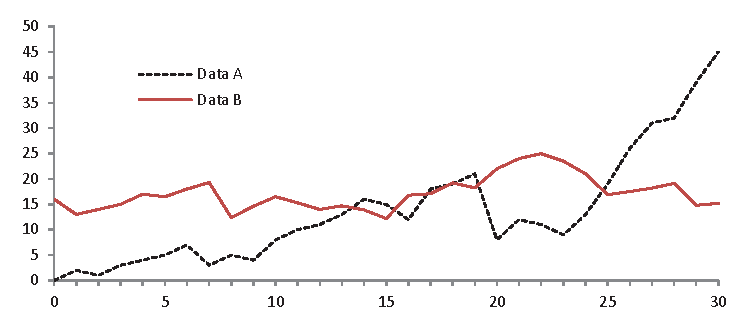
\includegraphics[width=\textwidth]{fig1.eps}
\caption{A figure caption is always placed below the illustration.
Please note that short captions are centered, while long ones are
justified by the macro package automatically.} \label{fig1}
\end{figure}

\begin{theorem}
This is a sample theorem. The run-in heading is set in bold, while
the following text appears in italics. Definitions, lemmas,
propositions, and corollaries are styled the same way.
\end{theorem}
%
% the environments 'definition', 'lemma', 'proposition', 'corollary',
% 'remark', and 'example' are defined in the LLNCS documentclass as well.
%
\begin{proof}
Proofs, examples, and remarks have the initial word in italics,
while the following text appears in normal font.
\end{proof}
For citations of references, we prefer the use of square brackets
and consecutive numbers. Citations using labels or the author/year
convention are also acceptable. The following bibliography provides
a sample reference list with entries for journal
articles~\cite{ref_article1}, an LNCS chapter~\cite{ref_lncs1}, a
book~\cite{ref_book1}, proceedings without editors~\cite{ref_proc1},
and a homepage~\cite{ref_url1}. Multiple citations are grouped
\cite{ref_article1,ref_lncs1,ref_book1},
\cite{ref_article1,ref_book1,ref_proc1,ref_url1}.
%
% ---- Bibliography ----
%
% BibTeX users should specify bibliography style 'splncs04'.
% References will then be sorted and formatted in the correct style.
%
% \bibliographystyle{splncs04}
% \bibliography{mybibliography}
%

\begin{thebibliography}{8}
% \bibitem{ref_article1}
%   Author, \href{https://scholar.google.com/citations?view_op=view_citation&hl=en&user=YFZ7DDkAAAAJ&citation_for_view=YFZ7DDkAAAAJ:Tyk-4Ss8FVUC}{Prashant Verma}, \emph{Title. Transitioning from Software Engineer to Engineering Manager (A Journey of Paradigm Shift)}.

\bibitem{prashant}
Author, Prashant Verma. Title. \emph{Transitioning from Software Engineer to Engineering Manager (A Journey of Paradigm Shift)}. Available online: \href{https://scholar.google.com/citations?view_op=view_citation&hl=en&user=YFZ7DDkAAAAJ&citation_for_view=YFZ7DDkAAAAJ:Tyk-4Ss8FVUC}{link}
  
\bibitem{anthony}
Author, Anthony Pellegrino. Title. \emph{Transitioning from Software Engineer to Engineering Manager[Online]}. Available:
\href{https://blog.tryexponent.com/transitioning-from-software-engineer-toengineering-manager/}{link}

\bibitem{matt}
Author, Mattheus Casparus Maree. Title. \emph{Engineering a manager: Assessing the factors affecting the career transition from engineer to manager}. Available:
\href{https://api.semanticscholar.org/CorpusID:209784964}{link}

\end{thebibliography}
\end{document}
